\documentclass[twoside,10pt]{article}
\usepackage{/Users/bradenhoagland/latex/styles/toggles}
%\toggletrue{sectionbreaks}
%\toggletrue{sectionheaders}
\newcommand{\docTitle}{HW 2}
\usepackage{/Users/bradenhoagland/latex/styles/common}
\importStyles{modern}{rainbow}{boxy}

%\renewcommand{\theenumi}{\alph{enumi}}

\begin{document}
%\tableofcontents

% ------------------------------
% 1
% ------------------------------
\begin{exer}
	(Hatcher 1.2: 1). Show that the free product $G * H$ of nontrivial groups $G$ and $H$ has trivial center, and that the only elements of $G * H$ of finite order are the conjugates of finite-order elements of $G$ and $H$.
\end{exer}

\textbf{Trivial center:} Let $x = x_1\dots x_{n}$ with $x_{n} \in G - \left\{ 1 \right\}$ be an element of $G * H$. Let $h \in H - \left\{ 1 \right\}$ be arbitrary, then $hx$ in reduced form ends with $x_n \in G$, but $xh$ in reduced form ends in $h \in H$. Thus $hx \neq xh$, so $x$ cannot be in the center of $G * H$. A similar argument holds if $x_{n} \in H- \left\{ 1 \right\}$ instead, so no nontrivial element of $G * H$ can be in the center.

Now the empty word, as the identity element, commutes with all other elements of $G * H$, so it is an element of the center. By the previous argument, it is the only such element, so the center of $G * H$ is trivial.

\textbf{Finite order $\implies$ conjugate:} First we show that any finite order element of $G * H$ is a conjugate of finite order elements of $G$ and $H$. Suppose $x = x_1 \dots x_m \in G * H$ has finite order, i.e. $x^{n}$ is the empty word for some $n \in \mathbb{N}$. This necessarily means 
\[
	\underbrace{(x_1\dots x_m)\dots(x_1 \dots x_m)}_{n \text{ times}} = \text{ the empty word}.
\] In order for this to reduce to the empty word, we need $x_{n-i} x_{i+1}=e$ for all $0 \leq i \leq m-1$. Then since left and right inverses coincide in groups, $x_{m-1} = x_{i+1}^{-1}$ for all $i$. We then have two cases:
\[
\begin{cases}
	(x_m^{-1} \dots x_{\lfloor m/2-1 \rfloor}^{-1}) \;x_{\lfloor m/2 \rfloor}\; (x_{\lfloor m/2+1 \rfloor} \dots x_{m}) & $m$ \text{ is odd} \\
	(x_m^{-1} \dots x_{m/2-1}) \;e\; (x_{m/2+1} \dots x_{m}) & $m$ \text{ is even}.
\end{cases}
\] 
Since $e$ is clearly of finite order, $x$ is the conjugate of a finite order element when $m$ is even. When $m$ is odd,
\[
e = x^{n} = x_{\lfloor m/2 \rfloor},
\] so $x$ is a conjugate of finite order $x_{\lfloor m/2 \rfloor}$.

\textbf{conjugate $\implies$ finite order:} Suppose $x g x^{-1}$ is an element of $G * H$, where $g$ is a finite order element of $G$ or $H$, i.e. $g^{n}=e$ for some $n \in \mathbb{N}$. Then
\[
	\underbrace{(xgx^{-1}) \dots (xgx^{-1})}_{n \text{ times}} = xg^{n}x^{-1} = xex^{-1} = x^{-1} = \text{ the empty word}
\] since all pairs $x^{-1}x$ give the identity and then are reduced away. Thus $xgx^{-1}$ has finite order $n$.

\newpage

% ------------------------------
% 2
% ------------------------------
\begin{exer}
	\color{white}.\color{black}
\begin{enumerate}
	\item (Hatcher 1.2: 4). Let $X \subset \mathbb{R}^3$ be the union of $n$ lines through the origin. Compute $\pi_1(\mathbb{R}^{3}-X)$.

	\item (Hatcher 1.2: 6). Use Proposition 1.26 to show that the complement of a closed discrete subspace of $\mathbb{R}^{n}$ is simply connected if $n \geq 3$.
\end{enumerate}
\end{exer}

\begin{enumerate}
	\item This argument assumes that all $n$ lines are disjoint. Obviously, if any two lines coincide, we can treat them as the same line and then we're working with $n-1$ lines instead of $n$.

		The map $F(x,t): (1-t)x + t \frac{x}{{\Vert{x}\Vert}} $ is a deformation retraction from $\mathbb{R}^{3}- X$ to $S^{2}$ minus $2n$ points, which shows that the two spaces are homotopy equivalent. Then since stereographic projection is a homeomorphism from $S^{n}-\left\{ \text{pt} \right\}$ to $\mathbb{R}^{n}$, the sphere minus $2n$ points is homeomorphic to $\mathbb{R}^{2}$ minutes $2n-1$ points. Then this space clearly deformation retracts onto the bouquet of $2n-1$ circles, so we have the sequence \[
			\mathbb{R}^{3}-X \quad\simeq\quad S^{2}- \left\{ 2n \text{ points} \right\} \quad\cong \quad \mathbb{R}^{2}- \left\{ 2n - 1 \text{ points} \right\} \quad\simeq\quad \underbrace{S^{1} \vee \dots \vee S^{1}}_{2n-1 \text{ times}} .
		\] 
		Then since the fundamental group of $m$ circles wedged together is the free product on $m$ generators, $\pi_1(\mathbb{R}^{3}-X)$ is the free group on $2n-1$ generators.

	\item \textbf{Trivial fundamental group:} Proposition 1.26 says that attaching any number of $3$-cells to a space does not affect the fundamental group. So suppose $X = \left\{ x_{\alpha} \right\}_{\alpha}$ is any closed discrete subspace of $\mathbb{R}^{n}$. Since it's discrete, by definition of the subspace topology, there must be open balls $B_{r_{\alpha}}(x_{\alpha})$ of $\mathbb{R}^{n}$ that intersect $X$ only at $x_{\alpha}$.

		Then the balls $B_{r_{\alpha}/2}(x_{\alpha})$ with radii halved are all disjoint. The space $\mathbb{R}^{n}-X$ is clearly a deformation retract of $\mathbb{R}^{n} - \{B_{r_{\alpha}/2}(x_{\alpha})\}_{\alpha}$, so they have isomorphic fundamental groups. But we can recover $\mathbb{R}^{n}$ from this space by filling in the holes with 3-cells, so by Proposition 1.26,
		\[
			1 \quad\cong\quad \pi_1(\mathbb{R}^{n}) \quad\cong\quad \pi_1\left( \mathbb{R}^{n} - \{B_{r_{\alpha}/2}(x_{\alpha})\}_{\alpha} \right) \quad\cong\quad \pi_1(\mathbb{R}^{n}-X).
		\] 

		\textbf{Path connected:} Suppose $\gamma$ is a path between two point in $\mathbb{R}^{n}$ that intersects $X$ at some points $\left\{ x_{\beta} \right\}_{\beta}$. As argued earlier, we can find disjoint open balls in $\mathbb{R}^{n}$ containing a single $x_{\beta}$ each. Then we can perturb $\gamma$ away from $x_{\beta}$ while staying in the open ball, giving us a path $\tilde{\gamma}$ between the same points that now doesn't intersect $X$. Thus $\mathbb{R}^{n}-X$ is path connected.
\end{enumerate}

\newpage

% ------------------------------
% 3
% ------------------------------
\begin{exer}
	(Hatcher 0: 14). Given positive integers $v,e$, and $f$ satisfying $v-e+f=2$, construct a cell structure on $S^2$ having $v$ 0-cells, $e$ 1-cells, and $f$ 2-cells.
\end{exer}

We can construct $S^2$ by taking a 0-cell and gluing the boundary of $D^2$ to it. Thus the sphere has $(v,e,f) = (1,0,1)$. Now consider the following two operations on $S^2$:
\begin{itemize}
	\item $\phi$: designate a point on $S^2$ to be a new 0-cell, and add a 1-cell between it and some other pre-existing 0-cell.
	\item $\psi$: Add a loop at some 0-cell.
\end{itemize}
\begin{figure}[H]
	\centering
	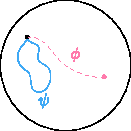
\includegraphics[scale=2]{fig/14.pdf}
	%\caption{}
\end{figure}

Note that $\phi$ adds a vertex and an edge, and $\psi$ adds an edge and a face, so both preserve the identity $v-e+f=2$. If $\phi$ is performed $a$ times and $\psi$ is performed $b$ times on the sphere, then we can represent the number of 0-cells, 1-cells, and 2-cells as
\[
	(1,0,1) + a(1,1,0) + b(0,1,1).
\] Suppose $(v,e,f)$ is an arbitrary triple satisying $v-e+f=2$, then if we let $a=v-1$ and $b=e-v-1$, this becomes
\[
	(v,e,2+e-v) = (v,e,f).
\] Since $\phi$ and $\psi$ both preserve $v-e+f=2$, we end up with our desired cell structure on $S^2$.

\newpage

% ------------------------------
% 4
% ------------------------------
\begin{exer}
Suppose $\Gamma$ is a 1-dimensional cell complex and let $E$ be an edge of $\Gamma$ connecting two different vertices (0-cells) of $\Gamma$, where $E$ includes both of its endpoints. Show that $\Gamma$ is homotopy equivalent to the quotient space $\Gamma/E$ obtained by shrinking $E$ to a point (don't use Hatcher's Proposition 0.17 or the homotopy extension property, etc).
\end{exer}

Since $E$ connects two different endpoints, it is clearly contractible. Thus there is a homotopy $F:E \times I\to E$ between $\id_{E}$ and $q$, the quotient map $\Gamma \epi \Gamma/E$. Now add some $1$-cell to $E$ to get a space $\tilde{E}$.

We can extend $F$ to all of $\tilde{E}\times I$ as follows:
\begin{itemize}
	\item First note that there is a retraction $r:D^{1}\times I \to (\p_{}{D^{1}}\times I) \uni (D^{n}\times \left\{ 0 \right\})$ given by radially projecting from the point $(0,2)$.
	\item We can let $F|_{D^1 \times 0}$ just be the identity.
	\item Now define $F|_{D^1 \times I}(x,t) = (F_t\circ r)(x)$. This is well-defined since it agrees with our original $F$ on $E\times I$ and since $r$ maps $D^1\times I$ into $(\p_{}{D^{1}}\times I) \uni (D^{1}\times \left\{ 0 \right\})$. This is a subset of $(E\times I) \uni (D^1 \times \left\{ 0 \right\})$, where $F$ is already defined.
\end{itemize}
Now extend this result by induction to all of $\Gamma$. This gives us a homotopy $G:\Gamma\times I \to \Gamma$. Since $G_1$ is constant on $E$, it induces a map $\psi:\Gamma/E \to \Gamma$ such that the following diagram commutes.
\[
\begin{tikzcd}
	\Gamma \rar{G_1}\dar[two heads]{q} & \Gamma \\
	\Gamma/E \arrow[ru,"\psi"']
\end{tikzcd}
\] 
We claim that $\psi$ and $q$ are maps showing $\Gamma \simeq \Gamma/E$. The homotopy $G_t$ shows $\id_{\Gamma} \simeq \psi q$, but the other direction is less straightforward.

Note that since $G_t(E) \subset E$ for all $t$, we have $qG_t(e_1) = qG_t(e_2)$ whenever $e_1, e_2 \in E$. Being in $E$ is exactly the equivalence relation determining the quotient space $\Gamma/E$, so by the universal property of quotient spaces, there is a unique $\tilde{G}_t$ making the following diagram commute.
\[
\begin{tikzcd}
	\Gamma \dar[two heads]{q} \arrow[dr, "qG_t"] \\
	\Gamma/E \rar[dashed, "\exists!\;\tilde{G}_t"'] & \Gamma/E.
\end{tikzcd}
\] 
Putting these diagrams together, we get
\[
\begin{tikzcd}
	\Gamma\dar[two heads]{q}\rar{G_t} & \Gamma \dar[two heads]{q} & & \Gamma \dar[two heads]{q}\rar{G_1} & \Gamma \dar[two heads]{q} \\
	\Gamma/E \rar["\tilde{G}_t"'] & \Gamma/E & & \Gamma/E \rar["\tilde{G}_1"']\arrow[ur,"\psi"] & \Gamma/E
\end{tikzcd}
\] Now $\tilde{G}_t$ is a homotopy between $\id_{\Gamma/E}$ and $q\psi$: $\tilde{G}_0 q = q G_0 = q$, which implies $\tilde{G}_0=\id_{}$ since $q$ is epic; $\tilde{G}_0q =qG_1=q\psi q$, which similarly implies $\tilde{G}_1 = q\psi$; and $\tilde{G}_t$ is continuous with respect to $t$ since $q G_t$ is.

Thus the quotient map $q$ is a homotopy equivalence showing $\Gamma \simeq \Gamma/E$.


\end{document}
